\documentclass[xelatex,aspectratio=169]{beamer}

\hfuzz=10pt
\vfuzz=10pt

% Theme
\usetheme{htw}
\setbeamertemplate{navigation symbols}{}
\setbeamertemplate{theorems}[numbered]
\setbeamercovered{transparent}

%\logo{
\includegraphics[height=0.5cm]{HTWD_color.png}}

% Packages
\usepackage{polyglossia}
\setmainlanguage{german}
\setotherlanguage{english}

\usepackage[bigfiles]{pdfbase}
\ExplSyntaxOn
\NewDocumentCommand\embedvideo{smm}{
\group_begin:
\leavevmode
\tl_if_exist:cTF{file_\file_mdfive_hash:n{#3}}{
  \tl_set_eq:Nc\video{file_\file_mdfive_hash:n{#3}}
}{
  \IfFileExists{#3}{}{\GenericError{}{File~`#3'~not~found}{}{}}
  \pbs_pdfobj:nnn{}{fstream}{{}{#3}}
  \pbs_pdfobj:nnn{}{dict}{
    /Type/Filespec/F~(#3)/UF~(#3)
    /EF~<</F~\pbs_pdflastobj:>>
  }
  \tl_set:Nx\video{\pbs_pdflastobj:}
  \tl_gset_eq:cN{file_\file_mdfive_hash:n{#3}}\video
}
%
\pbs_pdfobj:nnn{}{dict}{
  /Type/RichMediaInstance/Subtype/Video
  /Asset~\video
  /Params~<</FlashVars (
  source=#3&
  skin=SkinOverAllNoFullNoCaption.swf&
  skinAutoHide=true&
  skinBackgroundColor=0x5F5F5F&
  skinBackgroundAlpha=0.75
  )>>
}
%
\pbs_pdfobj:nnn{}{dict}{
/Type/RichMediaConfiguration/Subtype/Video
/Instances~[\pbs_pdflastobj:]
}
%
\pbs_pdfobj:nnn{}{dict}{
/Type/RichMediaContent
/Assets~<<
/Names~[(#3)~\video]
>>
/Configurations~[\pbs_pdflastobj:]
}
\tl_set:Nx\rmcontent{\pbs_pdflastobj:}
%
\pbs_pdfobj:nnn{}{dict}{
  /Activation~<<
  /Condition/\IfBooleanTF{#1}{PV}{XA}
  /Presentation~<</Style/Embedded>>
  >>
  /Deactivation~<</Condition/PI>>
}
%
\hbox_set:Nn\l_tmpa_box{#2}
\tl_set:Nx\l_box_wd_tl{\dim_use:N\box_wd:N\l_tmpa_box}
\tl_set:Nx\l_box_ht_tl{\dim_use:N\box_ht:N\l_tmpa_box}
\tl_set:Nx\l_box_dp_tl{\dim_use:N\box_dp:N\l_tmpa_box}
\pbs_pdfxform:nnnnn{1}{1}{}{}{\l_tmpa_box}
%
\pbs_pdfannot:nnnn{\l_box_wd_tl}{\l_box_ht_tl}{\l_box_dp_tl}{
  /Subtype/RichMedia
  /BS~<</W~0/S/S>>
  /Contents~(embedded~video~file:#3)
  /NM~(rma:#3)
  /AP~<</N~\pbs_pdflastxform:>>
  /RichMediaSettings~\pbs_pdflastobj:
  /RichMediaContent~\rmcontent
}
\phantom{#2}
\group_end:
}
\ExplSyntaxOff


\usepackage{graphicx}
\usepackage[export]{adjustbox}
\usepackage{animate}
%\usepackage[dvipdfmx]{movie15_dvipdfmx}
\usepackage{media9}
\usepackage{tabularx}
\usepackage{colortbl}
\usepackage{booktabs}
\usepackage{makecell}
\usepackage{ltablex}
\usepackage{array}
\usepackage{multirow}
\usepackage{amsmath}
\usepackage{amsthm}
%\renewcommand{\arraystretch}{1.5}
\newcolumntype{L}[1]{>{\raggedright\let\newline\\\arraybackslash\hspace{0pt}}p{#1}}
\newcolumntype{C}[1]{>{\centering\let\newline\\\arraybackslash\hspace{0pt}}p{#1}}
\newcolumntype{R}[1]{>{\raggedleft\let\newline\\\arraybackslash\hspace{0pt}}p{#1}}
%\renewcommand\thesatz{\arabic{section}.\arabic{theorem}}
\makeatletter
\@addtoreset{theorem}{lecture}
\makeatother

\newtheorem{satz}{Satz}[section]
\newtheorem{lem}{Lemma}[section]
\newtheorem{beh}{Behauptung}[section]
\newtheorem{define}{Definition}[section]
\numberwithin{equation}{section}
\usepackage{ragged2e}
\usepackage{etoolbox}

\usepackage{color}
\usepackage{colortbl}
\definecolor{hellgrau}{rgb}{0.85,0.85,0.85}
\definecolor{hellrot}{rgb}{1,0.7,0.7}

\usepackage{tikz}
\usetikzlibrary{shapes,arrows.meta,calc,arrows,positioning,patterns,tikzmark}
%\usepackage{tikz-uml}
\usepackage{pgfplots}  % for elliptic curves (part 8)
\pgfplotsset{compat=1.18}
\usepackage{pgffor}
\usepackage{pgfmath-xfp}
\tikzset{>=latex}
\tikzset{
  invisible/.style={opacity=0},
  visible on/.style={alt={#1{}{invisible}}},
  alt/.code args={<#1>#2#3}{%
      \alt<#1>{\pgfkeysalso{#2}}{\pgfkeysalso{#3}} % \pgfkeysalso doesn't change the path
    },
}

\usepackage{paralist}

\usepackage{url}
\def\UrlBreaks{\do\/\do-}
\PassOptionsToPackage{hyphens}{url}\usepackage{hyperref}

\usepackage[normalem]{ulem} % gestrichelte Unterstreichung (\dashuline{})
\usepackage{cancel}

\makeatletter
\renewcommand{\itemize}[1][]{%
  \beamer@ifempty{#1}{}{\def\beamer@defaultospec{#1}}%
  \ifnum \@itemdepth >2\relax\@toodeep\else
    \advance\@itemdepth\@ne
    \beamer@computepref\@itemdepth% sets \beameritemnestingprefix
    \usebeamerfont{itemize/enumerate \beameritemnestingprefix body}%
    \usebeamercolor[fg]{itemize/enumerate \beameritemnestingprefix body}%
    \usebeamertemplate{itemize/enumerate \beameritemnestingprefix body begin}%
    \list
    {\usebeamertemplate{itemize \beameritemnestingprefix item}}
    {\def\makelabel##1{%
        {%
            \hss\llap{{%
                  \usebeamerfont*{itemize \beameritemnestingprefix item}%
                  \usebeamercolor[fg]{itemize \beameritemnestingprefix item}##1}}%
          }%
      }%
    }
  \fi%
  \beamer@cramped%
  \justifying% NEW
  %\raggedright% ORIGINAL
  \beamer@firstlineitemizeunskip%
}
\makeatother

\apptocmd{\frame}{}{\justifying}{}

\renewcommand\theadfont{\bfseries\sffamily}
\usepackage{ragged2e}
\usepackage{newpxtext}

\setsansfont{texgyreheros}[
  Scale=MatchLowercase,
  UprightFont=*-regular,
  BoldFont=*-bold,
  ItalicFont=*-italic,
  BoldItalicFont=*-bolditalic,
]

% Title
\usepackage[usetransparent=false]{svg}
% Import references
\usepackage[backend=biber,style=numeric,sorting=none]{biblatex}
\addbibresource{references.bib}

%\AtBeginSection[]{
%  \begin{frame}
%    \vfill
%    \centering
%    \begin{beamercolorbox}[sep=8pt,center,shadow=true,rounded=true]{title}
%      \usebeamerfont{title}\thesection.~\secname\par%
%    \end{beamercolorbox}
%    \vfill
%  \end{frame}
%}

\makeatletter
\newenvironment{noheadline}{
  \setbeamertemplate{headline}{}
  \addtobeamertemplate{frametitle}{\vspace*{-0.9\baselineskip}}{}
}{}
\makeatother


\usepackage{xcolor}
\usepackage{algorithm}
\usepackage[linesnumbered,ruled,lined,commentsnumbered,algo2e,ngerman,ngermankw]{algorithm2e}
\usepackage{algorithmic}
\usepackage{caption}
\usepackage[newfloat]{minted}
\captionsetup[listing]{position=top}
\definecolor{mintedbg}{HTML}{282828}
\setminted{
  breaklines=true,
  bgcolor=mintedbg,
  style=monokai,
  formatcom=\color{white}
}
\usepackage{etoolbox}
\makeatletter
% replace \medskip before and after the box with nothing, i.e., remove it
\patchcmd{\minted@colorbg}{\medskip}{}{}{}
\patchcmd{\endminted@colorbg}{\medskip}{}{}{}
\makeatother

\renewcommand{\theFancyVerbLine}{\textcolor{black}{\arabic{FancyVerbLine}}}

\usepackage{pifont}
\newcommand{\cmark}{\ding{51}}%
\newcommand{\xmark}{\ding{55}}%

\newenvironment{changemargin}[2]{%
  \begin{list}{}{%
      \setlength{\topsep}{0pt}%
      \setlength{\leftmargin}{#1}%
      \setlength{\rightmargin}{#2}%
      \setlength{\listparindent}{\parindent}%
      \setlength{\itemindent}{\parindent}%
      \setlength{\parsep}{\parskip}%
    }%
    \item[]}{\end{list}}


\usepackage{csquotes}

% Title
\title{Algorithmen}
\author{Prof. Dr. Lukas Iffländer}
\institute{HTW Dresden}
\date{}
\usepackage{svg}

% Begin document
\begin{document}

% Title slide
\begin{frame}
  \titlepage
\end{frame}

\begin{frame}{Was ist ein Algorithmus?}{Motivation}
  Täglich führen wir Dinge nach festen Handlungsvorschriften aus:
  \begin{itemize}
    \item Bedienungsanleitung (z.B. für Kaffeemaschine)
    \item Montageanleitungen (z.B. für IKEA-Möbel)
    \item Verhaltensvorschriften (z.B. für soziale Interaktionen)
    \item Rezepte (z.B. für Kuchen)
    \item Rechenvorschriften (z.B. für Addition)
  \end{itemize}

\end{frame}

\begin{frame}{Was ist ein Algorithmus?}
  \begin{definition}
    Ein Algorithmus ist eine Vorschrift zur Lösung einer Klasse von
    Problemen. Er besteht aus einer endlichen Folge von Schritten,
    mit der aus bekannten Eingangsdaten neue Ausgangsdaten eindeutig berechnet werden können.
  \end{definition}

  \begin{block}{Eigenschaften}
    \begin{itemize}
      \item Definition zeigt engen Zusammenhang zu mathematischen Funktionen (Eingabe, Ausgabe)
      \item Definition bindet den Algorithmus an eine Klasse von Problemen nicht an eine einzelne Aufgabe
    \end{itemize}
  \end{block}

  \begin{alertblock}{Problem}
    \begin{itemize}
      \item Die Definition eines Algorithmus enthält keine Forderungen an die praktische Ausführbarkeit des Algorithmus auf einer realen Maschine (z.B. Computer)
    \end{itemize}
  \end{alertblock}
\end{frame}

\begin{frame}{Algorithmen als mathematische Funktionen}
  Ein Algorithmus kann als mathematische Funktion aufgefasst werden:
  \[ y = f \left(x\right) \mbox{ oder } f: D \rightarrow Z, x \rightarrow y \]
  \[ D: \mbox{Definitionsmenge}, Z: \mbox{Zielmenge} \]

  \begin{definition}
    In der Mathematik ist eine Funktion oder Abbildung eine Beziehung zwischen zwei Mengen, die jedem Element der einen Menge (Funktionsargument, unabhängige Variable, x-Wert) genau ein Element der anderen Menge (Funktionswert, abhängige Variable, y-Wert) zuordnet.
  \end{definition}
  \begin{block}{Interpretation}
    \begin{itemize}
      \item Element aus Mengen: Eingabe und Ausgabe
      \item Die Elemente können auch Mengen, Vektoren, Matrizen, etc. sein
    \end{itemize}
  \end{block}
\end{frame}

\begin{frame}{Berechenbarkeit}
  Somit wird einer Funktion ein Algorithmus zugeordnet.

  Es gibt aber Funktionen, denen kein Algorithmus zugeordnet werden kann. Diese Funktionen sind damit nicht berechenbar.

  \begin{definition}
    Eine Funktion $f$ heißt berechenbar, wenn es einen Algorithmus gibt, der für jedes Argument $x$ den Funktionswert $f\left(x\right)$ berechnet.
  \end{definition}

  \begin{exampleblock}{Beispiel}
    Ein einfaches Beispiel für eine berechenbare Funktion ist die Addition: $f\left(x\right) = x + 1$.
  \end{exampleblock}

  Weitere Beispiele folgen auf den nächsten Folien.

\end{frame}


\begin{frame}{Berechenbarkeit}{Beispiel: Sieb des Eratosthenes}
  \begin{block}{Problem}
    Finde alle Primzahlen bis zu einer gegebenen Zahl $n$.
  \end{block}

  \begin{block}{Algorithmus}
    \begin{enumerate}
      \item Erstelle eine Liste aller Zahlen von 2 bis $n$.
      \item Setze $p = 2$.
      \item Streiche alle Vielfachen von $p$ aus der Liste.
      \item Setze $p$ auf die nächste ungestrichene Zahl in der Liste.
      \item Wiederhole Schritte 3 und 4, bis $p^2 > n$.
      \item Die verbleibenden Zahlen in der Liste sind die Primzahlen.
    \end{enumerate}
  \end{block}

  \begin{exampleblock}{Zusatzübung}
    Implementierung als Python-Programm.
  \end{exampleblock}
\end{frame}

\begin{frame}{Berechenbarkeit}{Beispiel: Diskrete Funktion}
  Bereche die Funktionswerte der Funktion
  \[
    f\left(x+1\right) = 2 ^ {f\left(x\right)} \mbox{ mit } f\left(0\right) = 0
  \]
  für \( 6 \leq x \leq 12 \).

  \only<2->{\inputminted[firstline=8]{python}{src/algorithmus_funktion_weglaufend.py}}

  \only<3->{\begin{alertblock}{Problem}
      Die Werte der Funktion sind so groß, dass sie nicht mehr verarbeitet werden können.
    \end{alertblock}}

\end{frame}

\begin{frame}{Berechenbarkeit}{Ackermannfunktion I}

  \begin{definition}
    Die Ackermannfunktion ist eine Funktion, die für zwei natürliche Zahlen $m$ und $n$ definiert ist. Sie ist rekursiv definiert durch:
    \[
      A\left(m, n\right) = \begin{cases}
        n + 1                                   & \mbox{falls } m = 0                    \\
        A\left(m-1, 1\right)                    & \mbox{falls } m > 0 \mbox{ und } n = 0 \\
        A\left(m-1, A\left(m, n-1\right)\right) & \mbox{falls } m > 0 \mbox{ und } n > 0
      \end{cases}
    \]
  \end{definition}

\end{frame}
\begin{frame}{Berechenbarkeit}{Ackermannfunktion II}

  \inputminted[firstline=8,lastline=16]{python}{src/algorithmus_ackermann.py}

  \begin{alertblock}{Problem}
    %Die Ackermannfunktion wächst sehr schnell und ist für größere Werte von $m$ und $n$ nicht mehr berechenbar.

    \begin{itemize}
      \item $A\left(3, 2\right) = 29$
      \item $A\left(3, 3\right) = 61$
      \item $A\left(4, 3\right)$ ist nach fünf Minuten noch nicht berechnet
    \end{itemize}


  \end{alertblock}
\end{frame}

\begin{frame}{Berechenbarkeit}{Niht berechenbare Funktion}
  \begin{block}{Problem}
    Es gibt Funktionen, die nicht berechenbar sind.
  \end{block}

  \begin{exampleblock}{Beispiel}
    \begin{itemize}
      \item \enquote{Berechne} alle reellen Zahlen zwischen 0 und 1.
      \item Es kann bewiesen werden, dass ein solcher Algorithmus nicht existiert.
    \end{itemize}
  \end{exampleblock}

  \begin{alertblock}{Problem}
    Es gibt keine allgemeine Methode, um zu entscheiden, ob eine Funktion berechenbar ist.
  \end{alertblock}

\end{frame}

\begin{frame}{Berechenbarkeit}{Schlussfolgerungen}
  \begin{itemize}
    \item Viele Funktionen sind berechenbar und praktisch anwendbar (z.~B. Sieb des Eratosthenes).
    \item Manche Funktionen sind unter realistischem Ressourcen- und Zeitaufwand nicht auf einem Rechner umsetzbar, obwohl sie prinzipiell berechenbar sind (z. B. die gezeigte diskrete Funktion und die Ackermannfunktion).
    \item Einige Funktionen sind prinzipiell nicht berechenbar (wie die Berechnung aller reellen Zahlen zwischen 0 und 1).
  \end{itemize}
  \Rightarrow Es ist zweckmäßig, an Algorithmen solche Forderungen zu stellen, dass sie auf realen Maschinen praktisch ausgeführt werden können.

\end{frame}

\begin{frame}{Charakteristische Eigenschaften von Algorithmen I}
  \begin{itemize}
    \item \textbf{Endlichkeit}

          Ein Algorithmus muss aus einer endlichen Anzahl von Lösungsschritten bestehen und nach Abarbeitung dieser endlich vielen Schritte nach einer endlichen Zeit das Ende erreichen.

    \item \textbf{Eindeutigkeit}

          Die einzelnen Schritte eines Algorithmus und ihre Aufeinanderfolge müssen eindeutig beschrieben sein.
    \item \textbf{Allgemeinheit}

          Ein Algorithmus darf nicht nur die Lösung einer speziellen Aufgabe (z.B. Lösung der Gleichung $x^2 + 2x + 1=0$) , sondern muss die Lösung einer Klasse von Problemen (z.B. die Lösung aller quadratischen Gleichungen $ax^2 + bx + c = 0$) beschreiben.
  \end{itemize}
\end{frame}

\begin{frame}{Charakteristische Eigenschaften von Algorithmen II}
  \begin{itemize}
    \item \textbf{Determiniertheit}

          Die mehrmalige Anwendung des Algorithmus mit denselben Eingangsdaten muss immer wieder dieselben usgangsdaten
          liefern.

          Hinweis: Es gibt auch nichtdeterministische Algorithmen
    \item \textbf{Effizienz}

          Ein Algorithmus muss möglichst wenig Ressourcen einer Maschine, d.h. möglichst wenig Rechenzeit und möglichst wenig Speicher in Anspruch nehmen.
  \end{itemize}
\end{frame}

\begin{frame}{Darstellung von Algorithmen}{Natürliche Sprache}
  Zur Darstellung von Algorithmen sind Grundelemente notwendig.
  \begin{exampleblock}{Beispiel: Lösung einer quadratischen Gleichung}
    \[ a x^2 + b x + c = 0 \]
    nach der Mitternachtsformel:
    \[ x_{1,2} = \frac{-b \pm \sqrt{b^2 - 4ac}}{2a} \]
  \end{exampleblock}

  Neben der Notation einzelner elementarer Aktionen/Anweisungen, wie z.~B. \enquote{Gebe die Werte der Koeffizienten $a, b, c$ ein}, sind auch Strukturen notwendig, die die zeitliche Ablauffolge darstellen
  \begin{enumerate}
    \item Gebe die Werte der Koeffizienten $a, b, c$ ein.
    \item Berechne die Diskriminante $d = b^2 - 4ac$.
  \end{enumerate}
  oder eine Entscheidung repräsentieren.
  \begin{itemize}
    \item Falls $d < 0$: \ldots
  \end{itemize}
\end{frame}

\begin{frame}{Darstellung von Algorithmen}{Liste in natürlicher Sprache}
  \vspace{-1em}
  \begin{columns}
    \begin{column}{.5\linewidth}
      \begin{enumerate}
        \item Gebe Werte der Koeffizienten $a,b,c$ ein
        \item Berechne $d = b*b - 4*a*c$
        \item Falls $d \geq 0$: setze fort mit Schritt 6
        \item Ausgabe: "Keine Lösung"
        \item Stop
        \item Berechne $x_1 = \frac{-b + \sqrt{d}}{2*a}$
        \item Berechne $x_2 = \frac{-b - \sqrt{d}}{2*a}$
        \item Falls $d > 0$: setze fort mit Schritt 11
        \item Ausgabe: "Eine Lösung: ",$x_1$
        \item Stop
        \item Ausgabe: "Zwei Lösungen: ",$x_1$, " und ", $x_2$
        \item Stop
      \end{enumerate}
    \end{column}
    \begin{column}{.5\linewidth}
      \begin{block}{enthaltene Strukturen}
        \begin{itemize}
          \item Sequenz, d.h. Abarbeitung in der Reihenfolge der Nummerierung
          \item Auswahl, d.h. Entscheidung zwischen verschiedenen Alternativen (Überspringen von Schritten)
        \end{itemize}
      \end{block}
      \begin{alertblock}{Achtung}
        In Python kann dies nicht direkt umgesetzt werden, da die Logik \enquote{setze fort mit Schritt x} nicht existiert. Python hat keine GOTO-Anweisung.
      \end{alertblock}
    \end{column}
  \end{columns}
\end{frame}

\begin{frame}{Darstellung von Algorithmen}{Formale Darstellung}
  Bei der Darstellung von Algorithmen liegt der Schwerpunkt vor allem auf der Darstellung der zeitlichen Ablauffolge, dem sogenannten Steuerfluss.

  \begin{block}{Theorem von Böhm und Jacopini (1966)}
    Jeder Algorithmus kann durch eine Kombination von Sequenz, Auswahl und Iteration dargestellt werden.
  \end{block}

  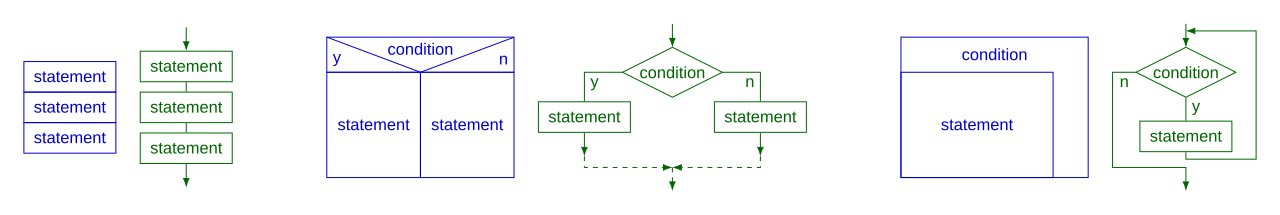
\includegraphics[width=\textwidth]{img/structured_program_patterns.png}
\end{frame}

\begin{frame}{Darstellung von Algorithmen}{Formale Darstellung -- Möglichkeiten}
  Es wurden zwei verschiedene Darstellungsformen entwickelt, die hauptsächlich in Gebrauch sind und auf grafische Symbole zurückgreifen:

  \begin{itemize}
    \item Früher Programmablaufplan (PAP) \rightarrow heute durch UML-Aktivitätsdiagramm ersetzt
    \item Struktogramm
  \end{itemize}

  Beide repräsentieren eine sogenannte Syntax, die die Ausdrucksformen der Beschreibung formal spezifiziert.

  Die Bedeutung der Darstellung wird als Semantik bezeichnet.
\end{frame}

% End document
\end{document}
